\section{Previous Work} 
Mainville \& Craymer (2005) used water gauge data collected around the LGL over the past 150 years to
 create monthly means of water level. Differences in these values between sites
 were then plotted against time to calculate a rate of elevation change between
 sites over time (This value being interpreted as the current impact of the GIA
 process on the crust underlying the LGL, although the actual process extends
 over a much longer timescale). Combinations of sites were shown to produce
 inconsistent results, so a second method using a least squares adjustment process was used,
 repeatedly removing some monthly mean outliers which fell some arbitrary residual distance away 
 from the linear regression line until none remained "too far away" from
 the final regression line. A third, and ultimately optimal method for calculating
 GIA was developed by
 Mainville \& Craymer in their 2005 paper, using the original
 method of directly comparing monthly
 water level means, but this time with adjustments for the epoch, site, and month of the year.
 Their findings with this method showed a general agreement with the post glacial
 ICE-3G global model of GIA at that time, while (Mainville \& Craymer, 2005).\\ \\
Johnston et al. (2012) attempted to provide a value for GIA in the LGL with
 better accuracy than previous estimates made using water
 gauge data. In order to accomplish this, the data used to measure the process of
 GIA needed to extend over a much longer timescale. In this method, water
 levels were inferred from the elevation of relict shorelines in beach ridge
 strandplains from the late Holocene sediment record surrounding Lake Superior,
 the ages for each data point being inferred from
 dating samples from these beach deposits (known as strandplain sequences) with
 Optically Stimulated Luminescence (OSL) age dating. This data differed from
 that used by Mainville \& Craymer in their 2005 paper, in that data collected did not have
 elevations sampled at the same points in time for calculation of relative
 rates. As a result, the elevation vs time data was modelled with a linear
 regression for each site, the difference in slopes representing the GIA rate
 between sites. Individual regressions were created per site
 for a series of four ranges of time related to lake level phases (Johnston et al, 2012). The results reported from this process
 are summarized in Figure \ref{fig:jj2012Grid}. \\
 
 \begin{figure}[t]
	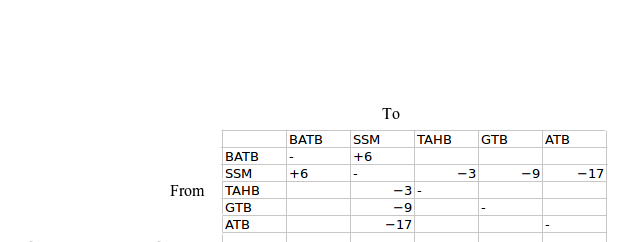
\includegraphics[width=0.9\linewidth]{jjGrid.png}
	\caption{GIA values reported by Johnston et al 2012. All values are in cm/century.}
	\label{fig:jj2012Grid}
 \end{figure}
 % need to ask JJ about JJ 2012, bottom of page 3, divergence of intercepts
 
